\section{Evaluating pacemaker software under all possible scenarios}
Testing has been the primary method to evaluate the safety and effectiveness of medical devices. During testing, a set of test cases are first specified which included an input sequence to the device and expected output sequence. Then the input sequence is feed into the device and the device output is compared with expected outputs from the test case. However, for closed-loop medical devices, there are infinite number of possible input sequences to the device. Exhaustively specifying all possible input sequences is unrealistic, thus safety violations of the devices may be omitted during testing.
Moreover, testing can only check whether the system is performing as specified, but cannot find safety violations with unknown executions.
\todo{KJ: I have a vague idea of what this means, but I think to an unknown reader this statement about safety violations with unknown executions will be confusing. Is this explained later?}

On the other hand, model checking is a technique that mathematically explore all possible executions of a model against specified requirements. Violations of the requirements are returned by the model checker tool as an execution trace, which can be analyzed and used to improve the system. Model checking has been widely used in the semi-conductor industry to verify chip design against their specifications.
Model checking is usually performed on a combined closed-loop models including the system under evaluation and a model of its environment. To capture the stochastic nature of the environment, certain transitions in the environment model are \emph{non-deterministic}, i.e. the next heart event can happen at any time within [0,500] msec. The model checker will explore all executions within the range for requirement violations.\todo[inline]{Limitations of model checking here?}

Model checking techniques can be used to evaluate the closed-loop model of the heart and the pacemaker against safety requirements. The aforementioned EP heart model uses timed-automata, which is suitable for various model checking tools.
With model checking, safety requirements can be specified in terms of avoiding safety hazards, so that model checker can potentially identify unknown mechanisms to induce safety hazards. A typical safety hazard of a pacemaker is pacemaker-mediated tachycardia, in which the pacemaker increase the heart rate inappropriately. The top figure in \figref{ambiguity} demonstrates the Endless-loop tachycardia (ELT), which is one case of pacemaker-mediated tachycardia. The ELT starts with an early ventricular contraction (PVC), which is a common scenario even in a healthy person. The electrical signal travels from the ventricle to the atrium (Red arrows in \figref{ambiguity}), triggering atrial sense (AS). The pacemaker paces the ventricle (VP) after a programed delay (AVI), which triggers ventricle to atrium conduction and this (AS-VP) pattern persists. The ventricular rate during ELT is determined by the conduction delay between the ventricle to the atrium and the programed delay in the pacemaker, which is very fast and do not change according to physiological need. 
To ensure the safety of the patient the ELT has to be eliminated. However, we also need to guarantee that only ELT has been eliminated without affecting other healthy heart functions.
The bottom figure in \figref{ambiguity} demonstrates a healthy condition with exact the same input-output sequence with ELT. The pacemaker pace the ventricle after each atrial event (AS) generated by the SA node, which maintains optimal blood flow. The heart model should be able to distinguish these two conditions in order to evaluate the new ELT-elimination algorithm. 

\begin{figure}[t]
		\centering
		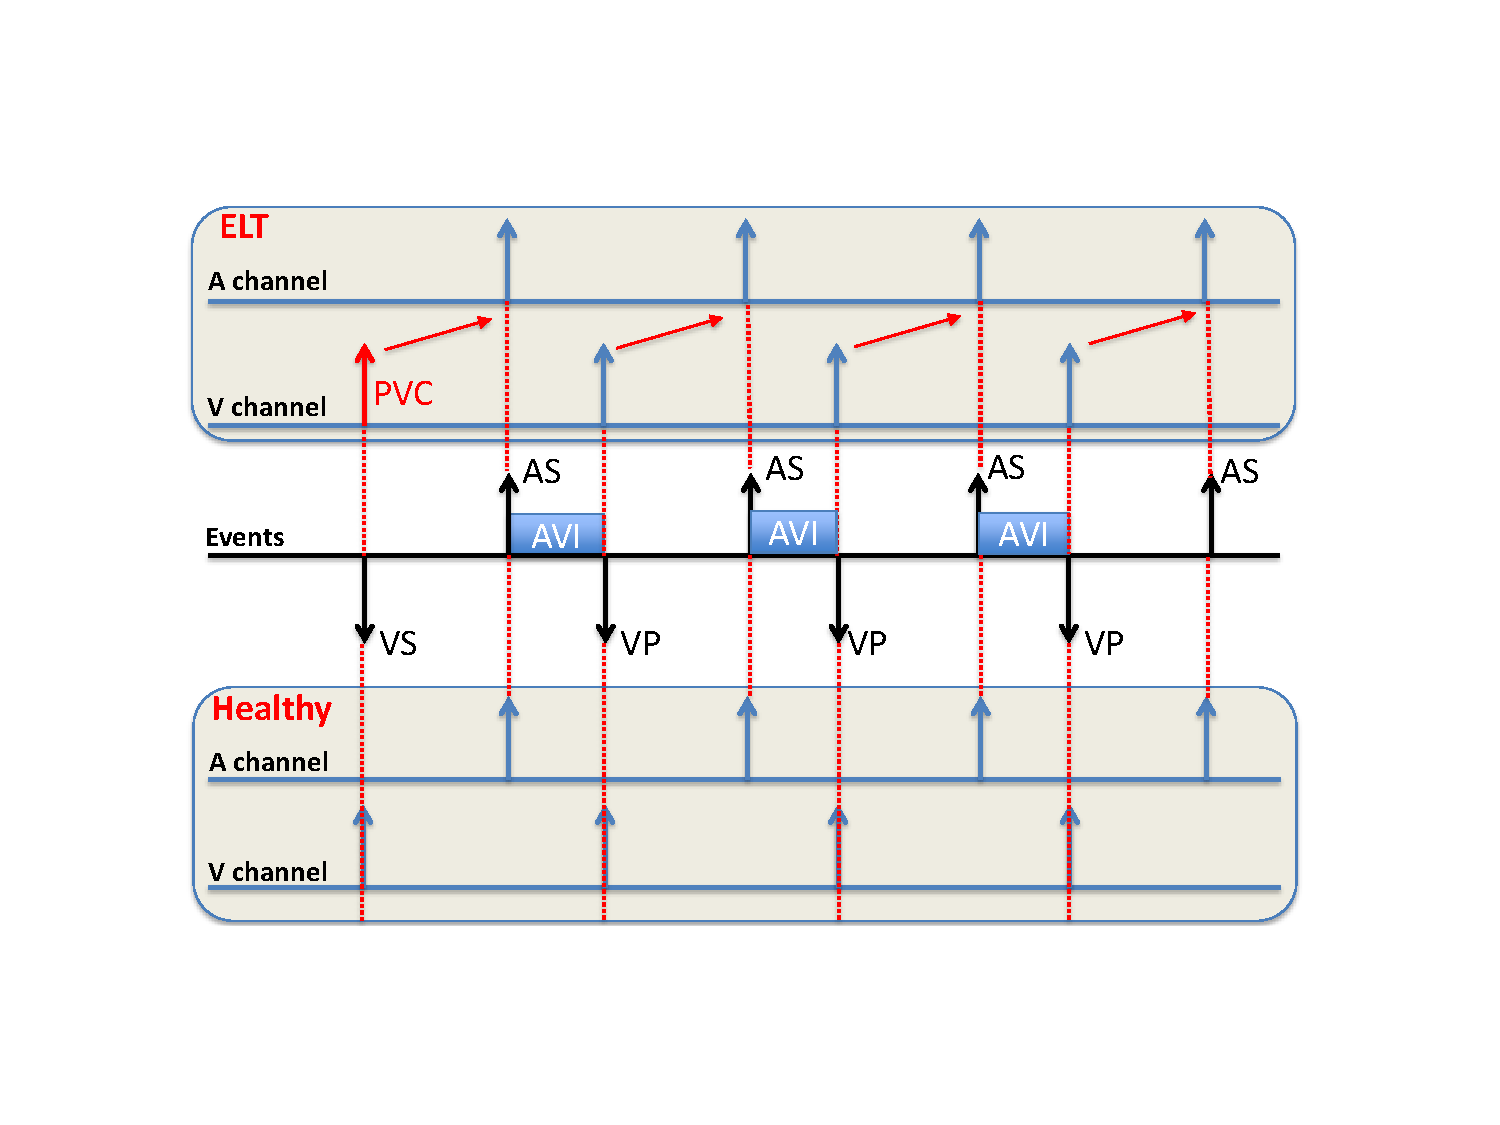
\includegraphics[width=\textwidth]{figs/ambiguity.pdf}
		\caption{\small Endless-loop Tachycardia (ELT) and a healthy heart condition mapped to the same input-output execution of the pacemaker (middle sequence). The heart model should have the details to resolve this ambiguity.}
		\label{fig:ambiguity}
\end{figure}
From the example above, we can see that in order to perform model checking on the closed-loop system, the heart model should not only cover all possible inputs to the pacemaker specified in the requirement, but also have enough details to resolve ambiguities of executions that may introduce false-positives and false-negatives. 
 \figref{abs_tree} demonstrates a collection of heart conditions modeled by the EP heart models. These models are definitely not exhaustive. Model checking the pacemaker model with all these heart models will not guarantee absolute safety. By using physiological abstraction rules (R1-R7 in \figref{abs_tree}), the heart conditions can be generalized and expand the possible inputs to the pacemaker. The result is a heart model $H_{all}$ with only two node automata correspond to the inputs to the pacemaker. By allowing both node automata to be able to send inputs to the pacemaker $[0,\infty]$msec after the last input, the heart model $H_{all}$ covers all possible inputs to the pacemaker. However, $H_{all}$ cannot distinguish the ELT condition from the healthy condition due to the lack of representation of ventricle to atrium conduction. The heart model $H_{cond}$ models the conduction between the atrium and the ventricle with a path automata, thus is the appropriate heart model to evaluate ELT.
%However, $H_{all}$ is not always the ultimate solution. For requirements that are condition-specific (i.e. Pacemaker should not increase heart rate when the heart rate is above certain threshold), $H_{all}$ do not have enough details to represent the corresponding condition in the requirement.
%Moreover, with structures corresponding to physiological components abstracted away, there exists executions from different heart conditions mapped to the same input-output sequence which cannot be distinguished. We can see that with heart model $H_{all}$ these two conditions cannot be distinguished. By adding a path automaton between the two node automata, the conduction direction can be distinguished, making the two conditions distinguishable. From this example we learn that choosing the correct heart model during model checking is essential to guarantee the validity of the model checking results. 

\begin{figure}[t]
		\centering
		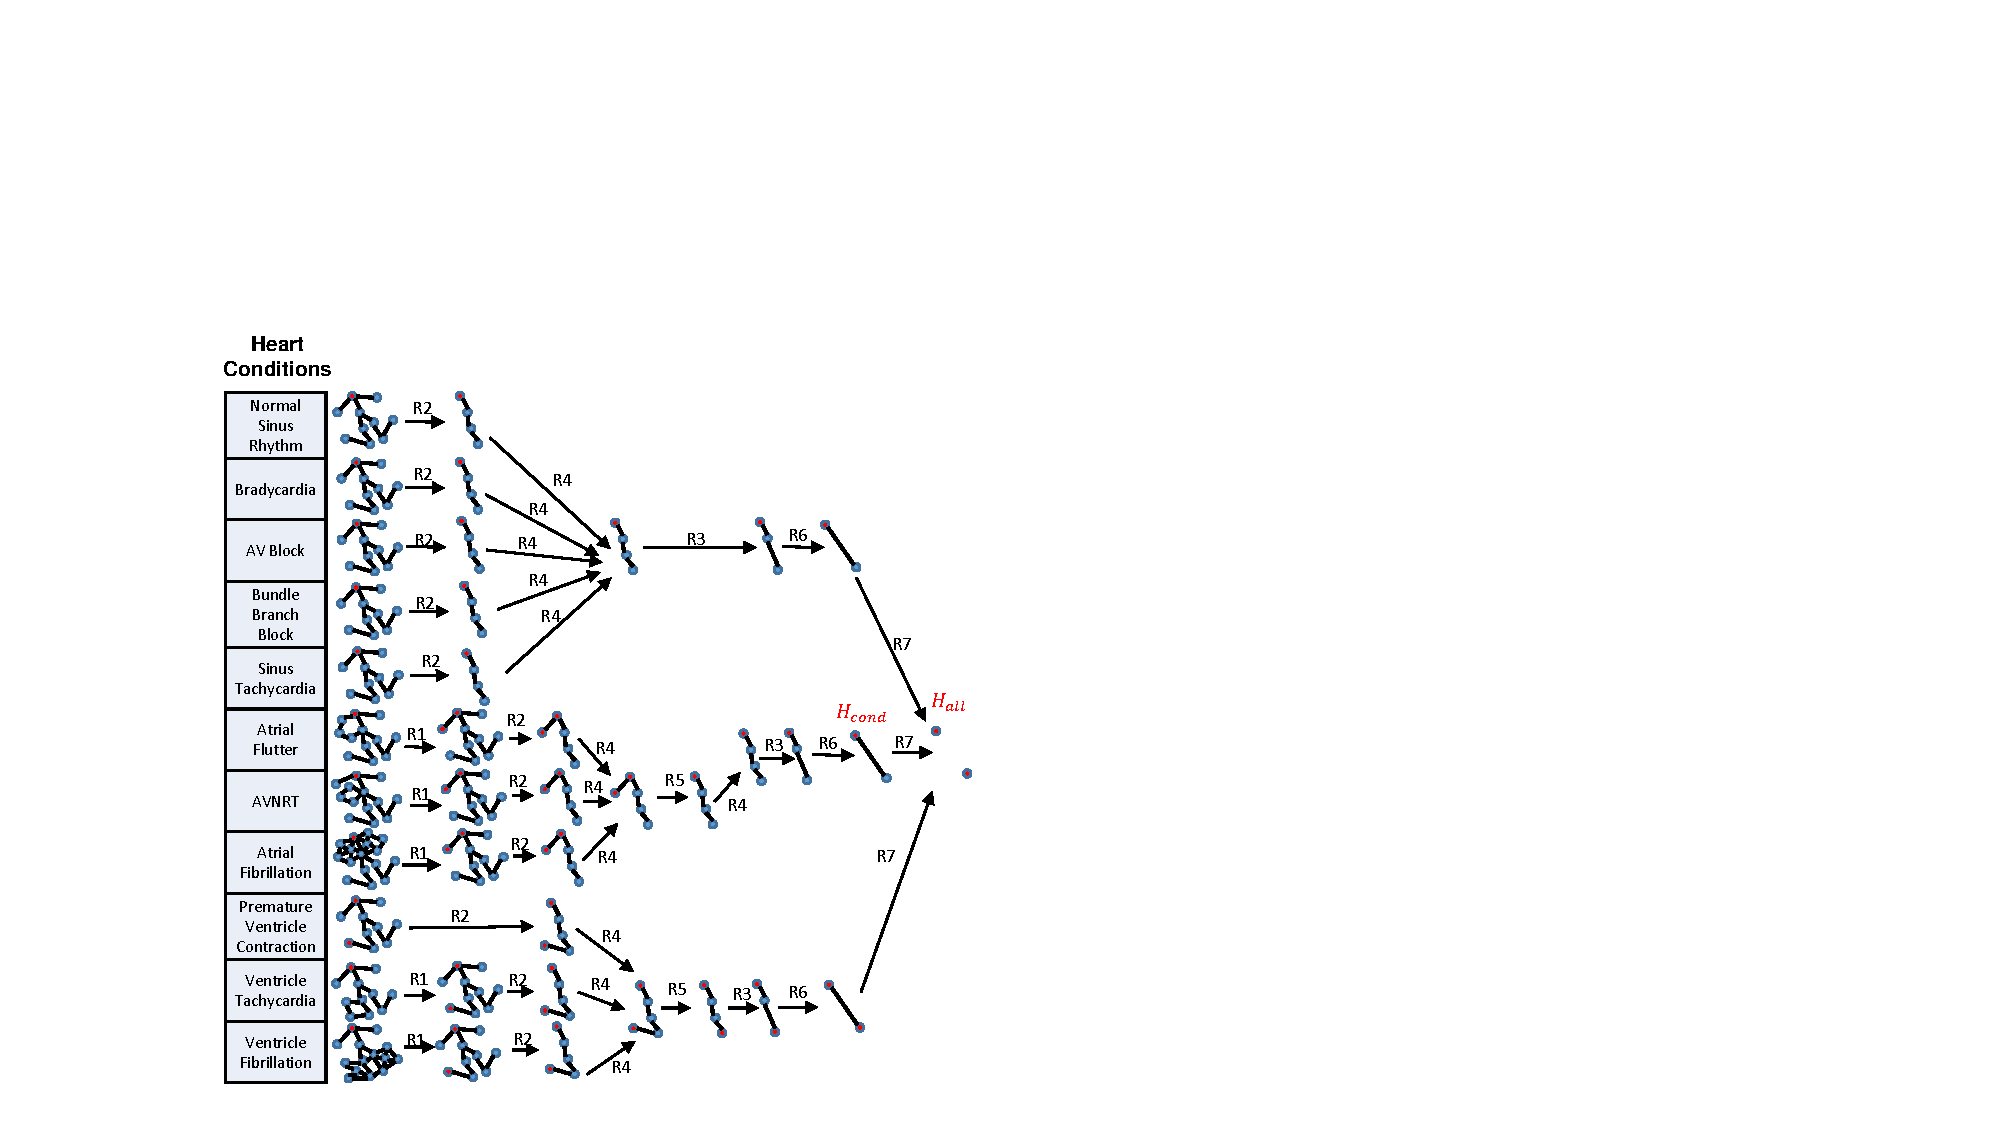
\includegraphics[width=\textwidth]{figs/abs_tree.pdf}
		\caption{\small Multi-scale modeling of the heart. The heart model at a higher level (further to the right) contains all possible inputs to the pacemaker from the heart models at previous levels}
		\label{fig:abs_tree}
\end{figure}

\section{Putting it all together}
During model checking, the abstract model of the pacemaker is validated against safety requirements. In the semi-conductor industry, the Verilog version of the chip design is model checked and automatically translated into logic gate implementation. 
\todo{I may be being picky, but after learning more about the automation tools, it isn't a completely automatic process to go from Verilog description to the chip.}
Similarly, the abstract pacemaker model can be automatically translated into simulation models and to code implementation (\figref{modelbaseddesign}). This automated translation provides rigorous traceability throughout the development process and ensures that the verified model is translated into verified code. The heart models are also available at simulation and implementation levels. 

\begin{figure}[t]
	\centering
	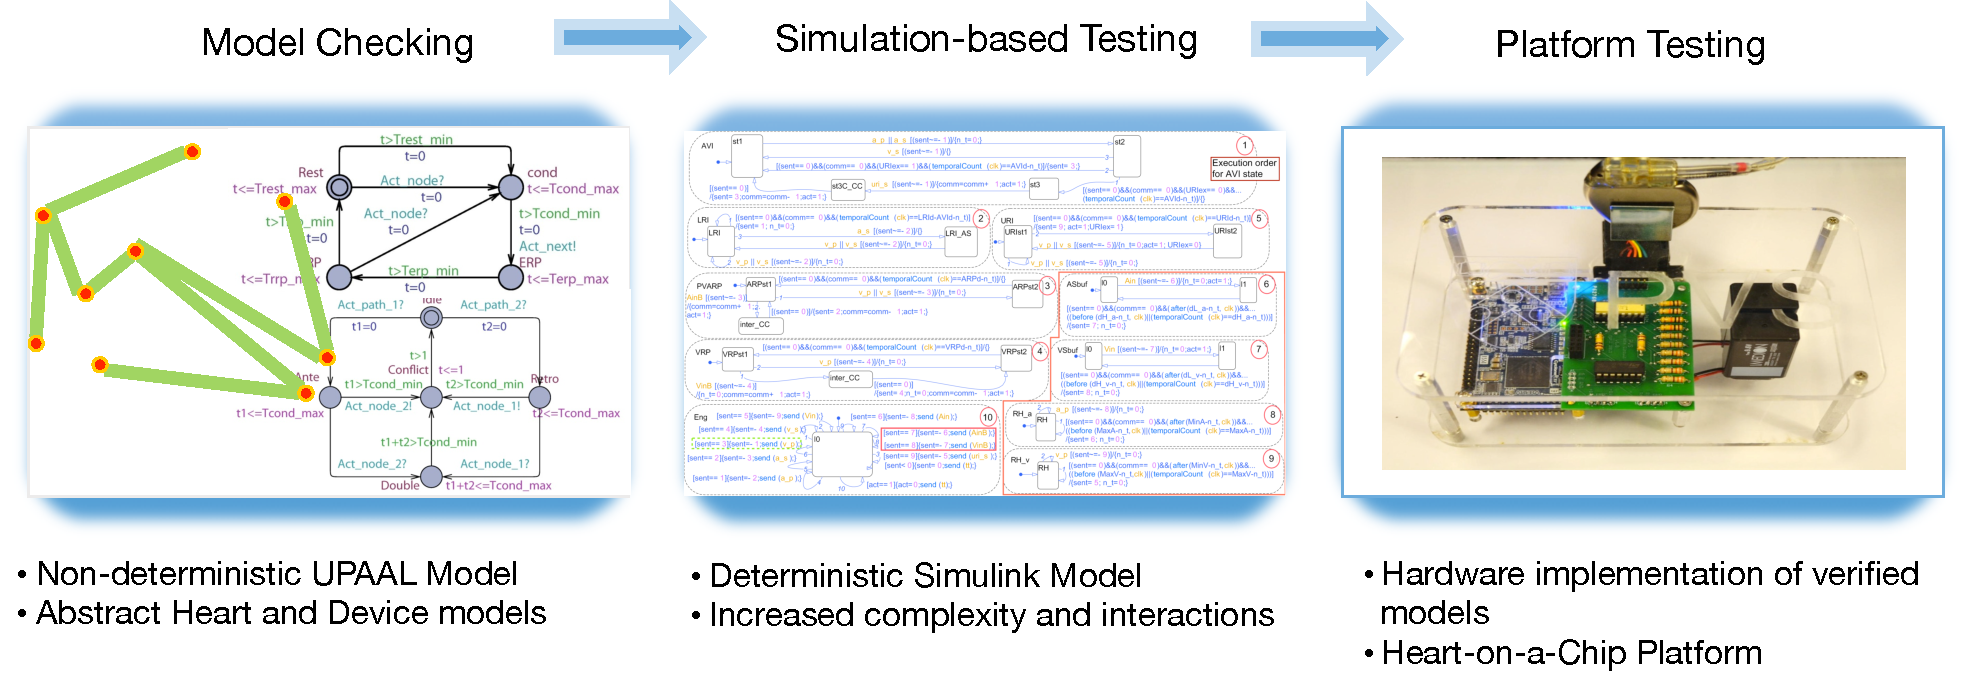
\includegraphics[width=\textwidth]{figs/fig4designtoimplementation.pdf}
	\caption{\small Model-based design framework. The pacemaker design is verified using model checking and automatically translated into code implementation. Heart models are available at all levels}
	\label{fig:modelbaseddesign}
\end{figure}
